\documentclass{article}

% Language setting
% Replace `english' with e.g. `spanish' to change the document language
\usepackage[english]{babel}

\usepackage[margin=1in]{geometry}

% Set page size and margins
% Replace `letterpaper' with `a4paper' for UK/EU standard size \usepackage[letterpaper,top=2cm,bottom=2cm,left=3cm,right=3cm,marginparwidth=1.75cm]{geometry}
% Useful packages
\usepackage{amsmath}
\usepackage{graphicx}
\usepackage{multirow}
\usepackage{booktabs}
\usepackage[colorlinks=true, allcolors=blue]{hyperref}
\usepackage{tikz}
\def\checkmark{\tikz\fill[scale=0.4](0,.35) -- (.25,0) -- (1,.7) -- (.25,.15) -- cycle;}

\title{Video Query Processing with Text}
\author{Sinclair Hudson}

\begin{document}
\maketitle

\begin{abstract}
      While LLMs are now frequently extended to process visual information in the form of images, they are not yet commonly used to process video.
      This work explores a general pipeline that leverages large language models (LLMs) to convert video into textual descriptions, and then further retrieve clips relevant to a query using those textual descriptions.
      The pipeline is called the VideoDescriptor pipeline, and is evaluated on text-to-video retrieval as well as video summarization.
      While not as accurate as other methods, the VideoDescriptor pipeline is able to achieve reasonable results on both tasks, and is completely zero-shot.
      Code for all experiments is available at \url{https://github.com/SinclairHudson/video-understanding}.
\end{abstract}

\section{Introduction}

The performance of language models has surged in recent years, largely thanks to the predictable scaling of transformer-based models.
In addition, multimodal vision-language models have been developed to create a shared latent representation between images and text \cite{clip} \cite{coca} \cite{mmbt}.
These multimodal models have enables zero-shot adaptation in many tasks, and have been merged with transformer-based language models to create large language models (LLMs) that can process visual information in the form of images \cite{flamingo} \cite{llava} \cite{gpt4vision} \cite{gemini}.
These LLMs, with the ability to understand both images and text, can now perform a lot of traditional benchmark tasks zero-shot, after being trained on vast amounts of semi-structured internet data \cite{gpt4vision} \cite{clip} \cite{gemini} \cite{flamingo}.
Despite their success in understanding images, LLMs have not yet shown the same success in understanding video.
Popular video understanding benchmarks such as MSR-VTT \cite{}, MSVD \cite{}, and ActivityNet \cite{} are still largely dominated by architectures custom-built for video understanding.
While these architectures often use the same techniques of self-supervised pre-training and further transfer learning, they do not use the same LLMs that have been so successful in image understanding.
This work proposes a general pipeline for accomplishing video understanding tasks using multimodal LLMs, by converting visual information into text and then completing the analog task in the text domain.



\section{Related Work}

\subsection{Video Understanding}

Video understanding is a difficult machine learning task, for many reasons.
The data is very high-dimensional and yet semantically sparse; most frames and pixels are redundant when analysing the video for content.
Additionally, video data is extremely time-consuming to annotate.
As such, very few video datasets exist, and are often much smaller than analogous image datasets \cite{imagenet} \cite{coco}.
Nevertheless, videos are ubiquitous in digital life, on popular social media websites like YouTube and TikTok. 
The research domain of video understanding is active and diverse.
Below, a few of the most relevant works are briefly introduced.

CLIP4Clip is a method that aims to extend the ideas of CLIP \cite{clip} to the video domain \cite{clip4clip}.
It generally follows a bi-encoder structure, in which the video and text are encoded using separate transformers \cite{transformer}.
The video is split into different patches spatially, and each patch is encoded using a linear layer into an embedding vector, and then processed by the video encoder transformer.
The text is tokenized and then processed by the text encoder transformer.
Then, both the video and text latent representations are fed into a similarity calculator module.
The system is trained end-to-end with video-text pairs and contrastive loss, as in CLIP \cite{clip}.
CLIP4CLip is naturally suited for video retrieval, since it can compute a similarity score between a video and a text query.
Given a text query, the system computes the similarity between the query and each video in the dataset, and retrieves the videos in order of similarity.

X-CLIP takes a similar approach to CLIP4Clip, using contrastive pre-training to learn associations between video and textual descriptions \cite{xclip}.
However, X-CLIP goes further and models more fine-grained associations between video and text.
For a given video-caption pair, the video is encoded frame-by-frame are then passed into a temporal encoder, producing both a vector for each frame and a vector for the entire video.
Likewise, the caption is encoded using a transformer, producing both a vector for the entire caption and a vector for each word.
X-CLIP explicitly models caption-video, caption-frame, word-video, and word-frame relationships, and uses these associations to learn very detailed representations of the video and text.
These representations, along with task-specific fine-tuning, allow X-CLIP to perform very well on text-to-video and video-to-text retrieval tasks.

InternVideo is a recent attempt at a ``foundation model" for video, being able to complete numerous downstream tasks.
The authors train InternVideo with a combination of multimodal contrastive learning (as in CLIP \cite{clip}), as well as masked video reconstruction, inspired by VideoMAE \cite{videomae}.
The InternVideo video encoder is pretrained on an unprecedently large dataset of internet videos and movies, allowing it to learn very semantically rich representations of videos.
This dataset is compiled by the authors using both pre-existing video datasets as well as videos scraped from the internet. In total, the dataset contains 12 million videos from 5 different domains \cite{internvideo}.
With additional fine-tuning on specific tasks, InternVideo achieves state-of-the-art performance on many action understanding, video-language alignment, and video open understanding benchmarks \cite{internvideo}.
Note that InternVideo is \textit{not} a large language model, though it uses the same strategy of large-scale, self-supervised pretraining.

\subsection{Large Language Models for Vision}

As mentioned in the introduction, it is now common to see LLMs that can process visual information in the form of images. 
Below are a few of the most relevant works that were designed, in part, to process multiple images at once.

Flamingo is a family of ``Visual Language Models", otherwise known as multimodal LLMs \cite{flamingo}.
In Flamingo models, image embeddings from an image encoder (ResNet without normalizers \cite{nfnet}) are introduced at every layer of a transformer-based language model.
The image encoder and language model are frozen, and only the cross-attention modules connecting the image features to the language features are trained for Flamingo.
This significantly reduces the computation required to train the system.
Flamingo is trained on many datasets, including image-text and video-text datasets. It is capable of taking as input multiple images or video frames. 
The authors note that adding relevant frames to the input incrementally improves performance on certain tasks, up to around 32 frames \cite{flamingo}.
This indicates that Flamingo is able to gather and aggregate useful features from many images simultaneously.

Like Flamingo, LLaVA \cite{llava} is a large language model trained on a combination of text-image and text-video data.
It is built upon the Vicuna language model \cite{vicuna}, and incorporates the visual encoder of CLIP \cite{clip} to encode images into embeddings that the language model can take as input.
It is fine-tuned end-to-end on instructional image-text data, and has proven to be exceptionally strong at visual question-answering tasks.
Due to the whole model being optimized end-to-end, LLaVA outperforms Flamingo on many tasks, but is also much more computationally expensive to train.
LLaVA is used in this work as the LLM for describing videos.

\subsection{Large Language Models for Video}

Most related to this work are attempts to leverage large language models for video understanding tasks.

VideoChat \cite{videochat} focuses on an understanding of video that is amenable to multiple-round video question answering.
VideoChat has two streams; VideoChat-Embed and VideoChat-Text.
VideoChat-Embed uses InternVideo to encode the video into a semantically meaningful vector representation.
VideoChat-Text uses multimodal language models to represent segments of the video as textual descriptions. 
These textual descriptions, in addition to the embedding from VideoChat-Embed, are fed into an LLM as context for question answering.

Video-ChatGPT \cite{videochatgpt} adapts LLaVA to process video instead of images.
The Video-ChatGPT pipeline can be broken down into 3 sequential modules: the visual encoder, the video embedding module, and the LLM.
Only the video embedding module is trained from scratch; the upstream visual encoder and downstream LLM remain frozen.
As such, Video-ChatGPT can be seen as a parameter-efficient fine-tuning approach to equip an LLM model with a visual encoder; the video embedding module adapts the visual encoder to video.
In their approach, the video embedding module embeds both frame-wise and spatial-patch-wise, allowing for the model to learn both temporal and spatial features.
Like VideoChat, Video-ChatGPT is largely designed for video question answering tasks and chat-like interactions.

\subsection{Video-Text datasets}
MSR-VTT (Microsoft Research Video to Text) is a flagship video understanding dataset \cite{msr-vtt}.
This dataset can be used for multiple tasks, including video question answering, video retrieval, and video captioning.
Every video in the dataset has multiple captions, each written by a different human annotator after watching the short video.
The dataset contains 10 000 videos, sourced from the internet by downloading video results of popular internet search queries.
For the video retrieval task, 1000 queries (video captions) are used for testing, each specifying exactly one video as the correct answer \cite{jsfusion}.
The videos in the video retrieval split are 14 seconds long on average, see Figure \ref{fig:length_histogram} for a histogram of video lengths.

\begin{figure}[h]
      \centering
      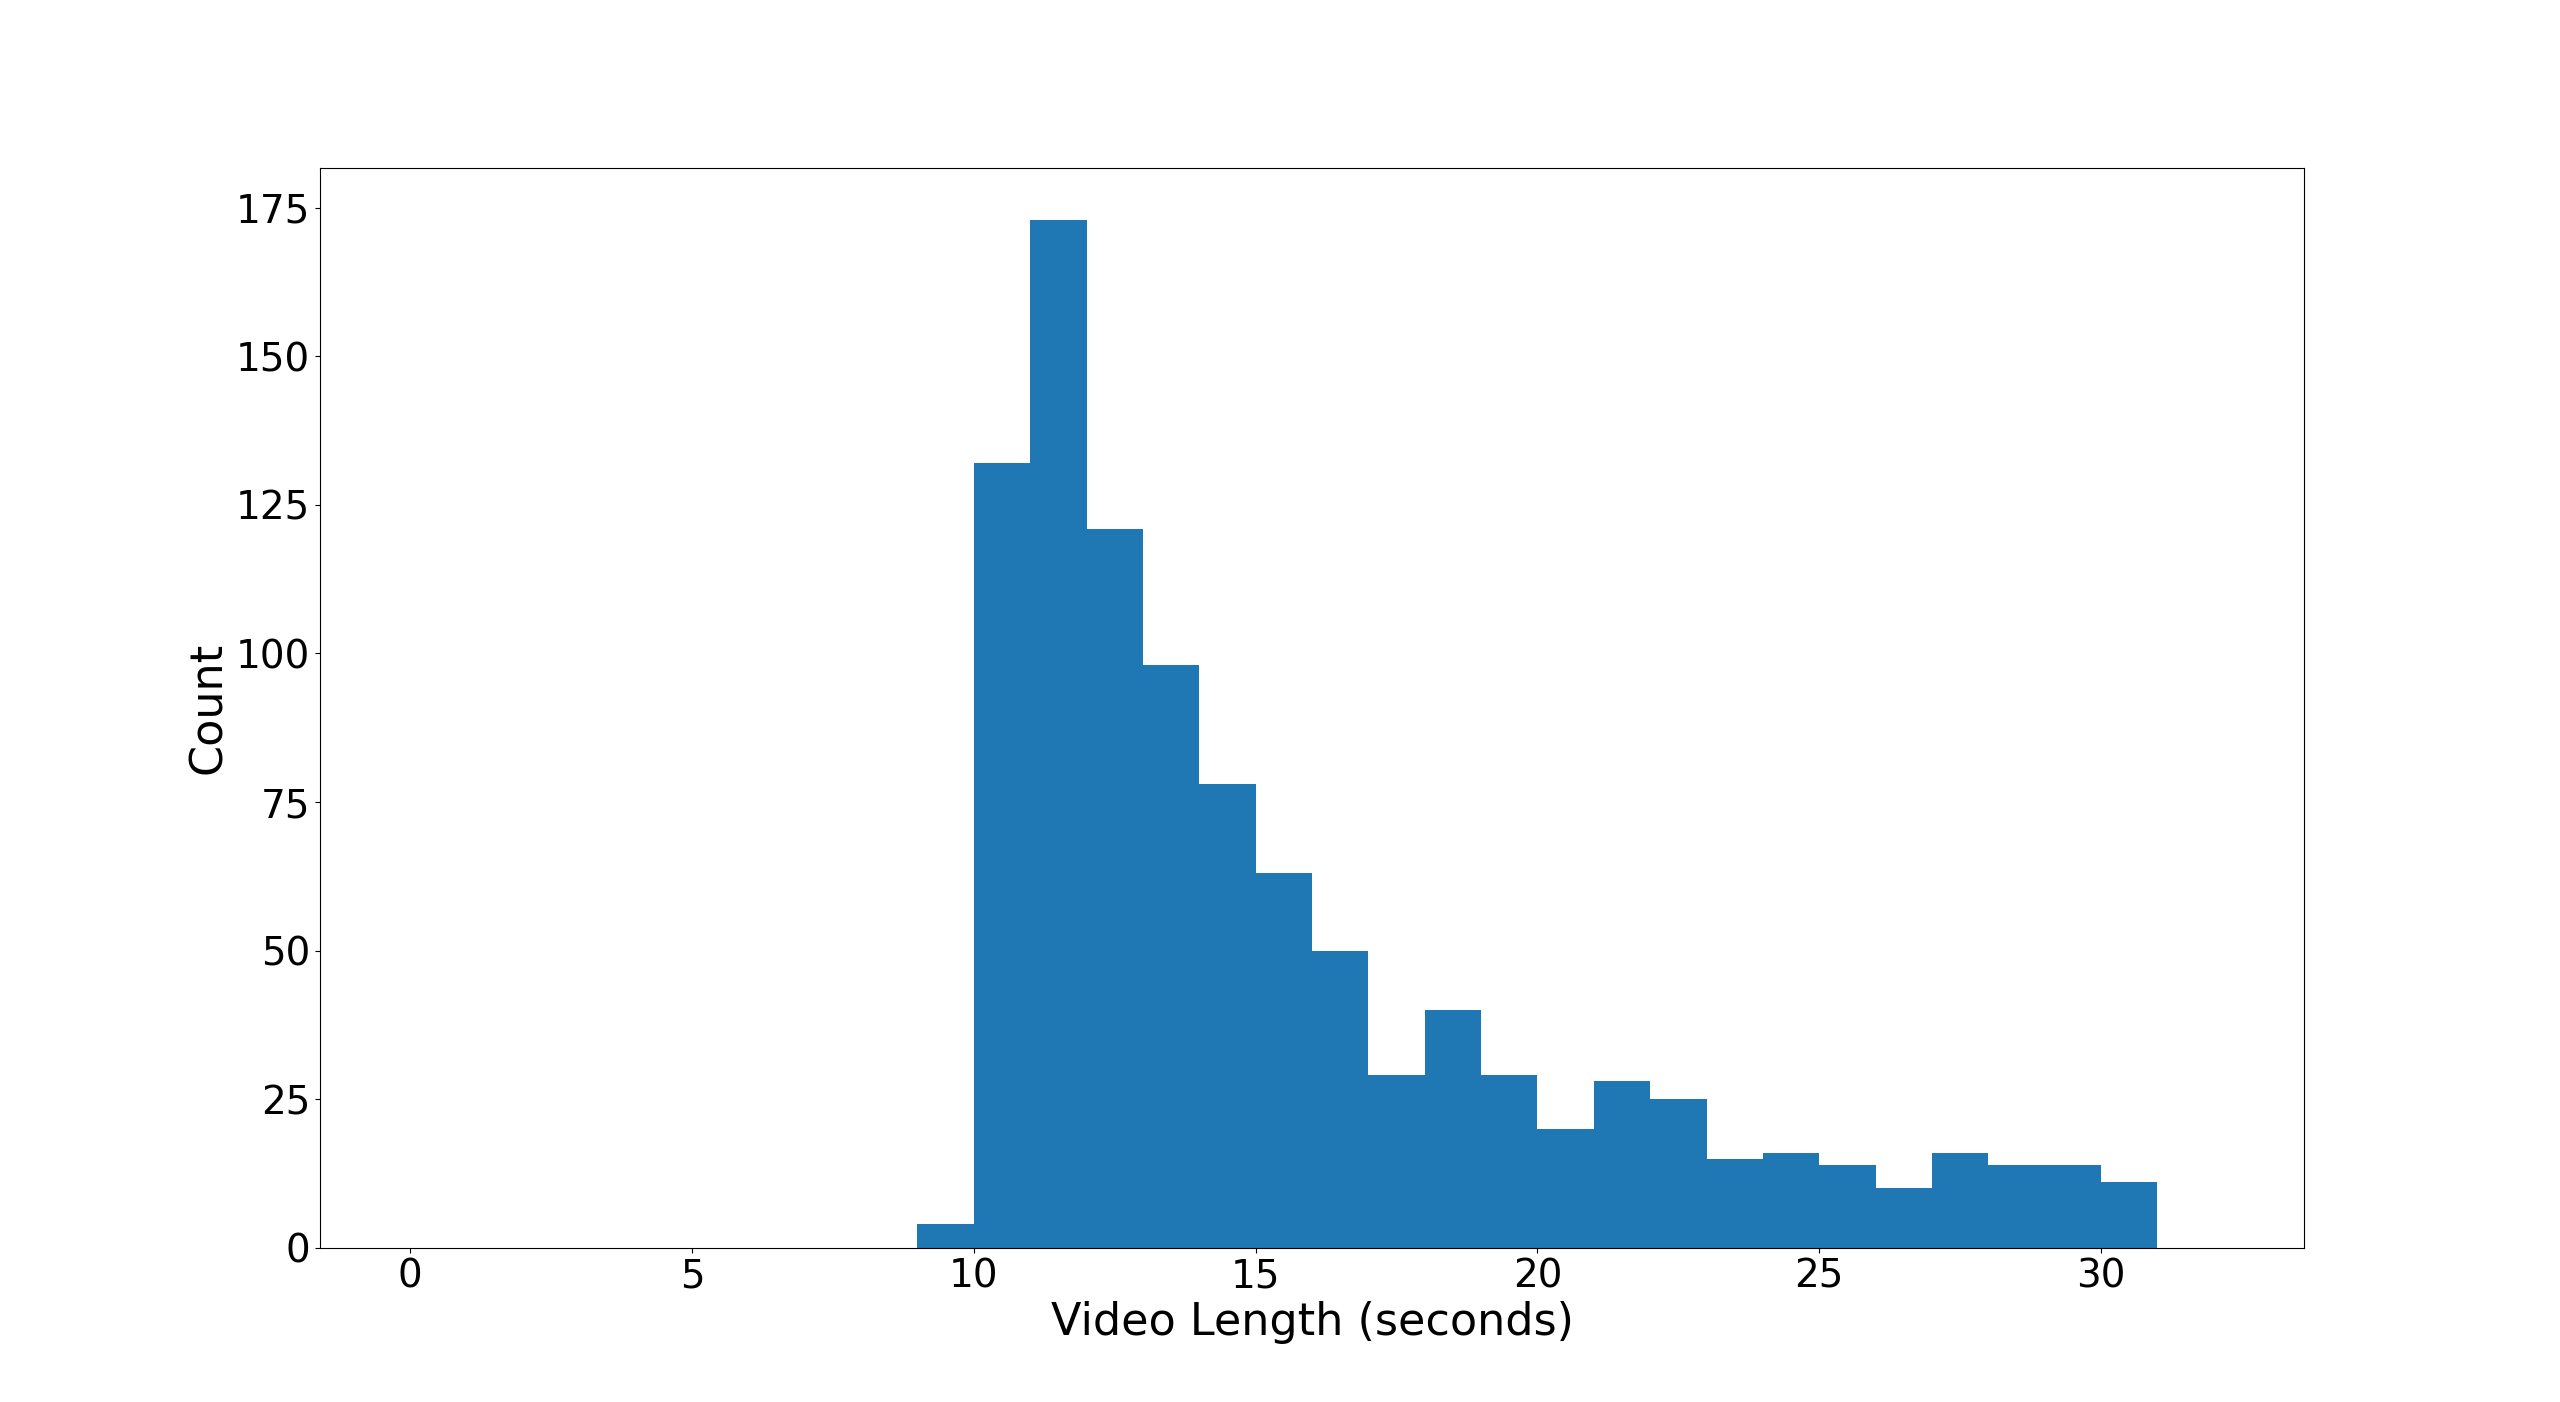
\includegraphics[width=0.7\textwidth]{figures/msr-vtt-length-histogram.png}
      \caption{Length of videos in the MSR-VTT retrieval data split.}
      \label{fig:length_histogram}
\end{figure}

While not used in this paper, other datasets like MSVD \cite{msvd} and ActivityNet \cite{activitynet} are also popular for video understanding tasks.
Microsoft Research Video Description Corpus (MSVD) is similar to MSR-VTT, consisting of short video clips and associated descriptions of the actions in the clip.
MSVD can be used for video captioning, video question answering, and video retrieval.
ActiviyNet is an extremely large dataset used for action classification (human activity understanding).
Given a video, the task is to classify the action being performed in the video, from a set of 200 classes.
ActivityNet version 1.3 contains 19994 videos from YouTube, making it one of the largest video datasets available.


\section{Method}


\begin{figure}
      \centering
      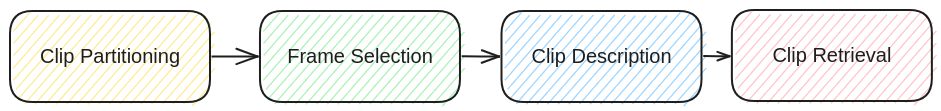
\includegraphics[width=0.8\textwidth]{figures/pipeline.png}
      \caption{High level block diagram of the proposed video understanding pipeline.}
      \label{fig:pipeline}
\end{figure}

The proposed pipeline is designed in such a way to be general to different video understanding tasks, with each of the 4 major steps allowing for multiple methods, or being optional for some tasks.
For the purposes of this work, a "clip" is a small segment of a video that is a few seconds long, 
and is highly cohesive in what it depicts. For example, in a movie, a clip might be a single shot.
At a high level, the pipeline for video understanding using LLMs is as follows:
\begin{enumerate}
      \item Partition the video into individual clips (optional)
      \item From each clip, select a small subset of frames to represent the clip
      \item Using the selected frames, generate a textual description of the clip using an LLM.
      \item Using the textual description, answer queries about the video, or retrieve clips.
\end{enumerate}

For brevity, these steps will be referred to as "Clip partitioning", "Frame selection", "Clip description", and "Clip Retrieval" respectively.
The two most applicable tasks for this pipeline are video retrieval and video summarization.
In video retrieval, given a query, the goal is to retrieve the video in a video dataset that best matches the query.
In visual video summarization, the goal is to edit a video down to a shorter length, containing only clips relevant to a given query.
Prior works often treat the video as-is and do not pre-process it much.



\section{Clip Partitioning}

Videos can contain a lot of different clips, which may or may not be related.
As such, it's desirable to process and describe each clip individually; clips are an atomic unit in video.
The input for clip partitioning is the whole video, and the output is a list of breaks (frame numbers) between clips.
The difficult aspect of clip partitioning is to efficiently find the boundaries between clips.
A two-hour video at 24 frames per second contains 172,800 frames, and so processing each one is computationally expensive.

The simplest approach to clip partitioning is to simply partition the video into equal-sized clips, without regard for the content of the video.
This approach is simple and fast to compute, but the resulting clips are not necessarily cohesive, since "clips" could contain multiple scenes and shots.

\subsection{Coarse-to-fine clip partitioning}
A more strategic approach identifies breaks as sequential frames with a large difference between them.
However, even computing a simple difference such as an L1 or L2 norm between each pair of frames is computationally expensive, since a norm must be taken per frame in the video.

As such, the VideoDescriptor pipeline uses a coarse-to-fine approach to clip partitioning.
The algorithm starts by computing the L1 distance between frames \textit{1 second apart}, over the entire video.
If the the L1 distance between these frames is above a certain threshold, then its likely that there's a clip break between them.
Thus, the 1-second segment is evaluated frame by frame, and if the distance between two frames is above the threshold, then a clip break is identified.
Empirically, this approach saves 60\% of the L1 computations compared to the naive frame-by-frame approach, and could save more if fewer coarse breaks are identified.

See Figure \ref{fig:breaks} for resulting clip breaks from the coarse-to-fine approach.
Qualitative results show that this approach is very effective at identifying clip breaks, with few false positives and false negatives.
Qualitatively, this approach struggles when large objects move quickly in the video, resulting in large differences between frames.
Sudden changes in the video, like the flash of a camera, are also often falsely identified as a clip break due to the sudden difference in brightness.

\begin{figure}
      \centering
      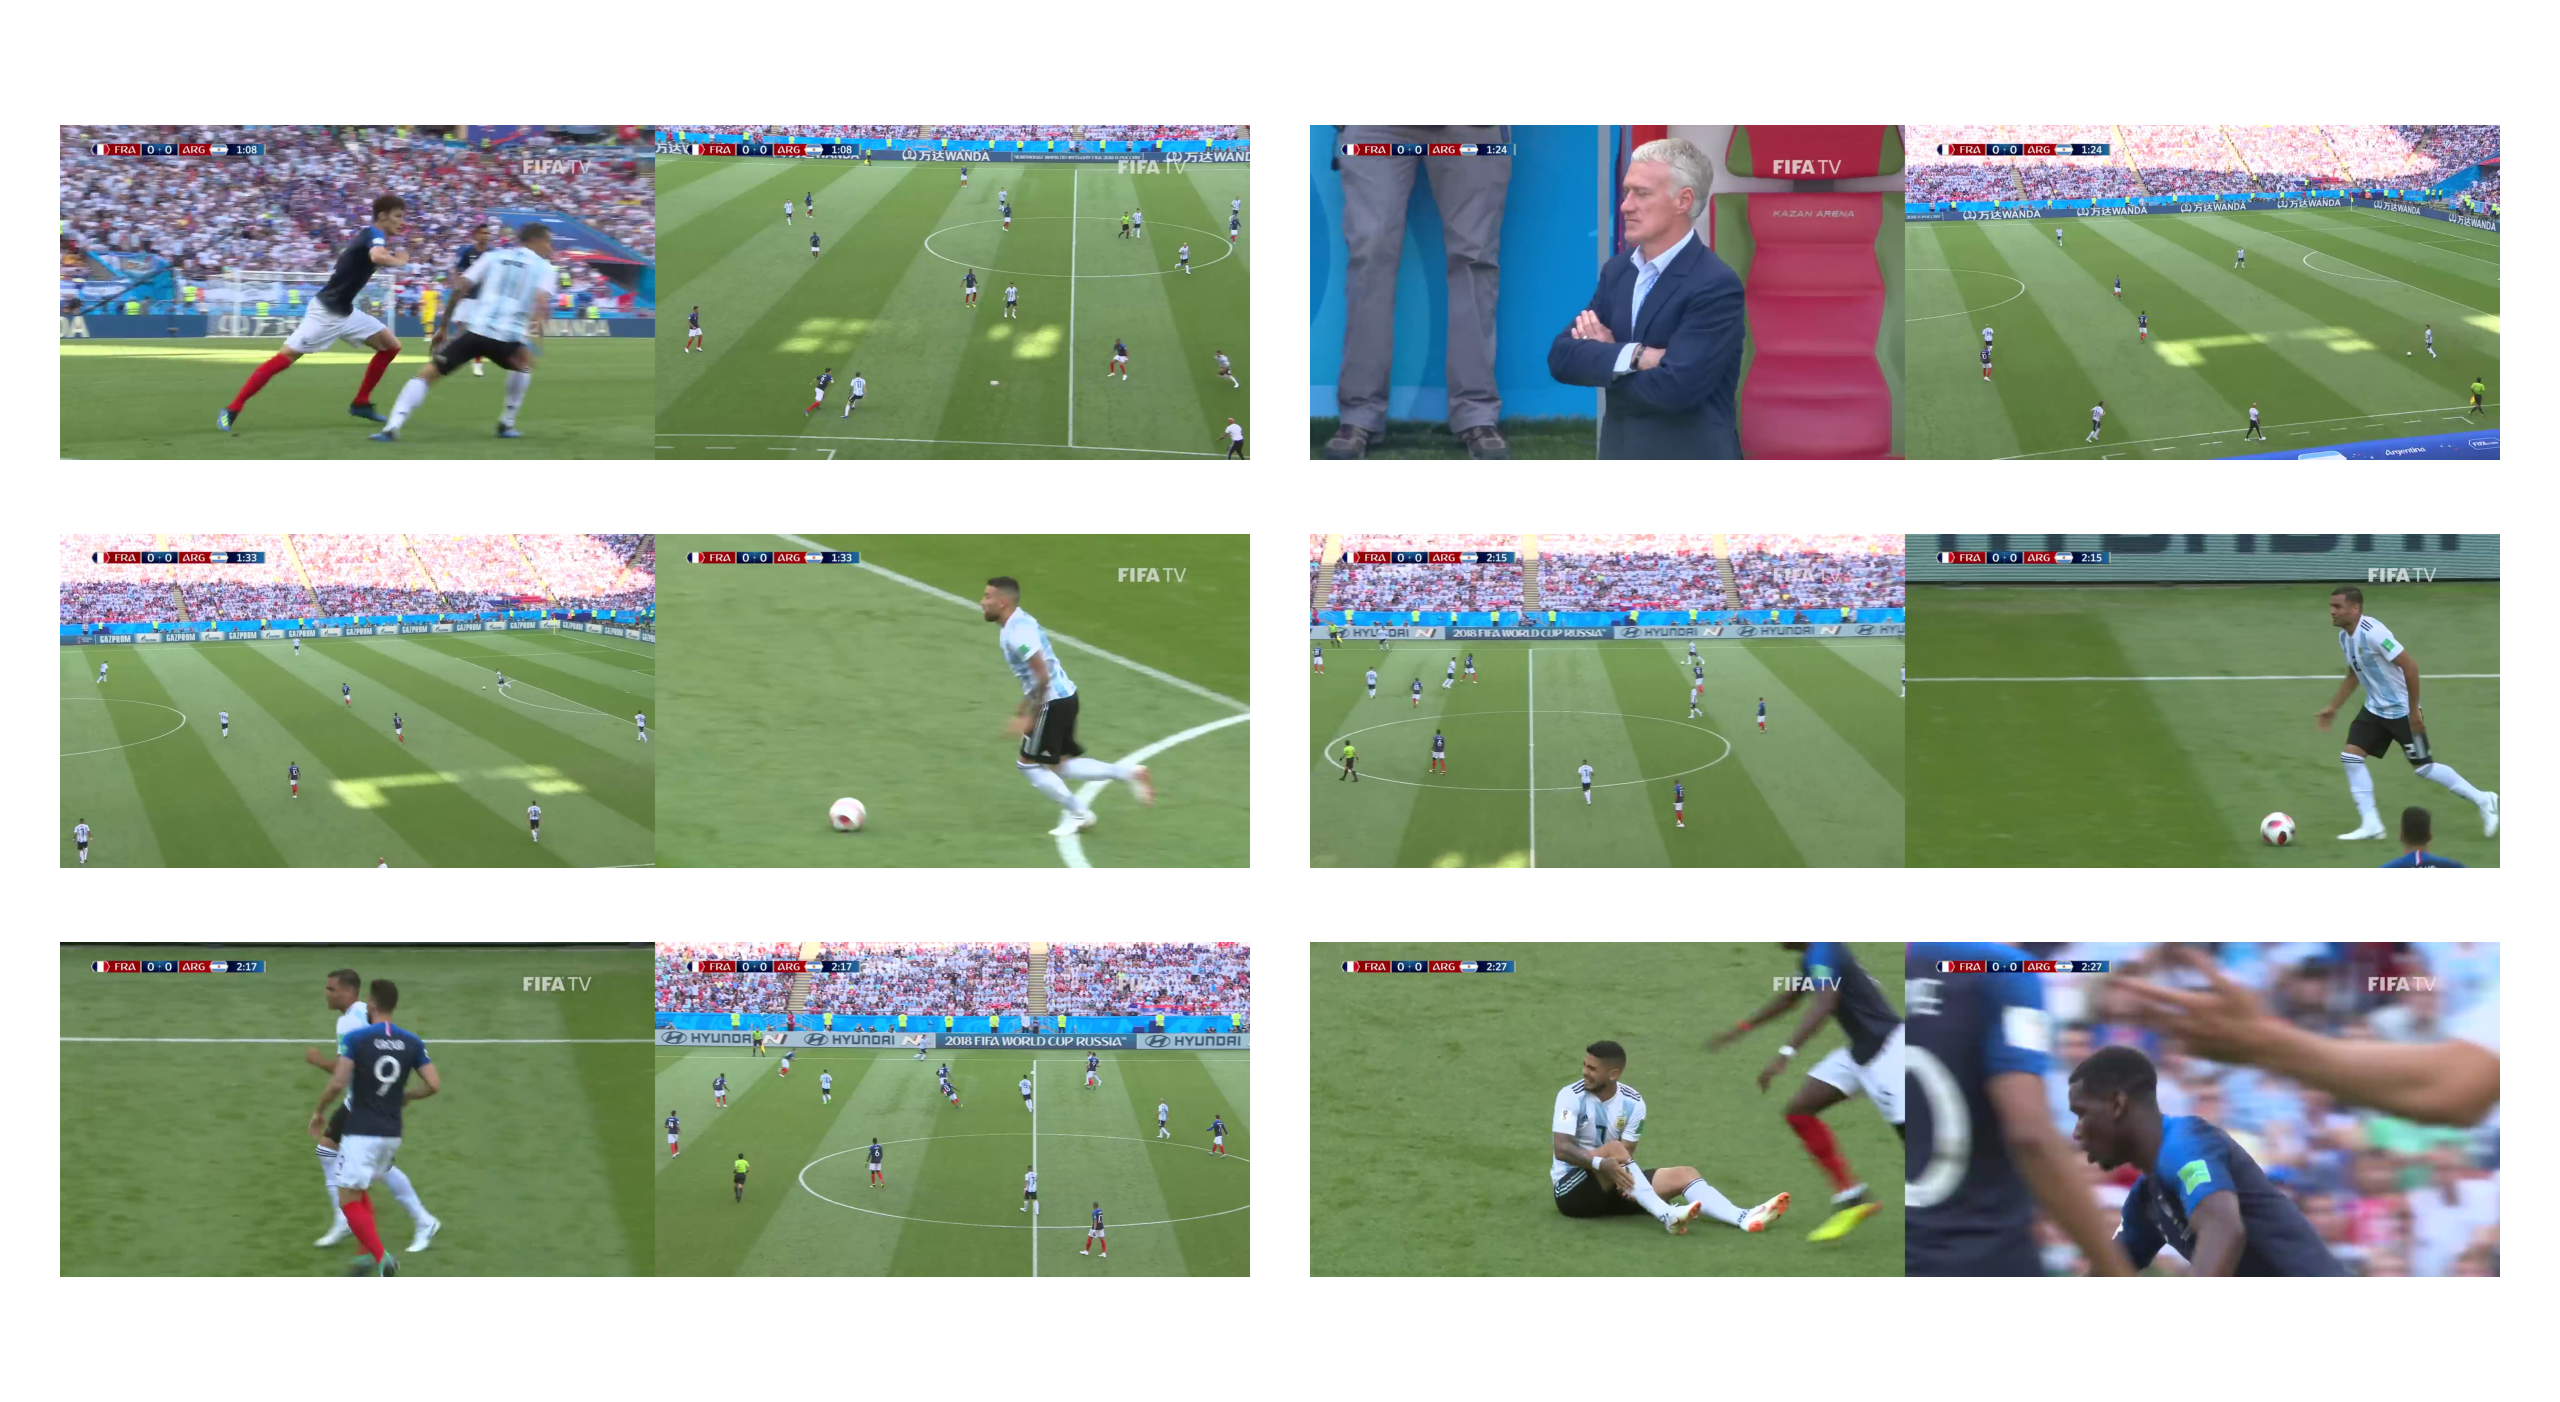
\includegraphics[width=\textwidth]{figures/breaks.png}
      \caption{Frames immediately before and after a clip break, determined by the coarse-to-fine clip partitioning strategy.}
      \label{fig:breaks}
\end{figure}


\section{Frame Selection}

Even within a single clip, there are a lot of frames, most of which are very similar to their neighbours.
To make the pipeline efficient, it's critical to select the subset of the most semantically relevant frames.
While some LLMs like LLaVA can take multiple images as input, they are rarely tested and likely not trained on multi-image inputs.
The input to frame selection is a clip (small length of video) and the output is a list of frames selected for further processing.

Earlier works simply sample randomly \cite{clipbert} or sample uniformly, at a course framerate such as 1 frame per second \cite{clip4clip}.

This work explores 3 different frame selection strategies:
greedy L1 selection, stratified sampling, random sampling, and stratified triplet sampling.

\subsection{Stratified Sampling}
To get a potentially more diverse set of frames, the first, last and middle frames are selected.
For brevity, this sampling method is referred to as \verb|3strat|. \verb|5strat| is also explored, which selects the first, last, and 3 evenly spaced frames in between.

\subsection{Random Sampling}
A random sampling approach is also explored, with either 3 or 5 frames selected from the video (with replacement).
These are referred to as \verb|3rand| and \verb|5rand| respectively.

\subsection{Stratified Triplet Sampling}
It's possible that the stratified sampling method above is too coarse, and that a single frames at multiple points in the clip is not enough to capture the clip's content.
For this reason, this work also explores stratified triplet sampling, where at each of the 3 points in the clip, 3 frames are selected across 1 second.
The motivation for this method is that the 3 frames in a single second will show what is changing in the scene.
each triplet is fed in as a single input into the LLM, which can take multiple images as input.
As a result, there is only one textual description per triplet in this sampling method.

\subsection{Greedy L1 Selection}
Greedy L1 selection initially selects the first frame of a clip. Then, it selects an additional clip if the L1 distance between the new frame and the previously selected frame is greater than some threshold (for example).
The L1 distance is normalized by the number of pixels in the image, so that the threshold is independent of the video resolution.
In the MSR-VTT dataset, most videos are quite short (see Figure \ref{fig:length_histogram}), and often only contain a single shot.
As such, when using Greedy L1 selection, a substantial number of videos only have the first frame selected (with L1 threshold 180).
The idea for selction based on L1 is to skip frames that are visually similar to the previously selected frame.
The selection strategy is greedy; the first frame is always selected, and then frames are considered in order, only selected if the frame differs from the previously selected frame by a certain L1 distance.
More formally

% TODO maybe just write an algorithm block for this? It's not difficult
\begin{equation}
      c < \frac{|I_{p} - I_{c}|}{W \times H \times C}
\end{equation}
where $c$ is a pre-defined threshold, $I_{p}$ is the previously selected frame, $I_{c}$ is the current frame, and $W$, $H$, $C$ are the width, height, and channels of the frames, respectively.

\begin{figure}
      \centering
      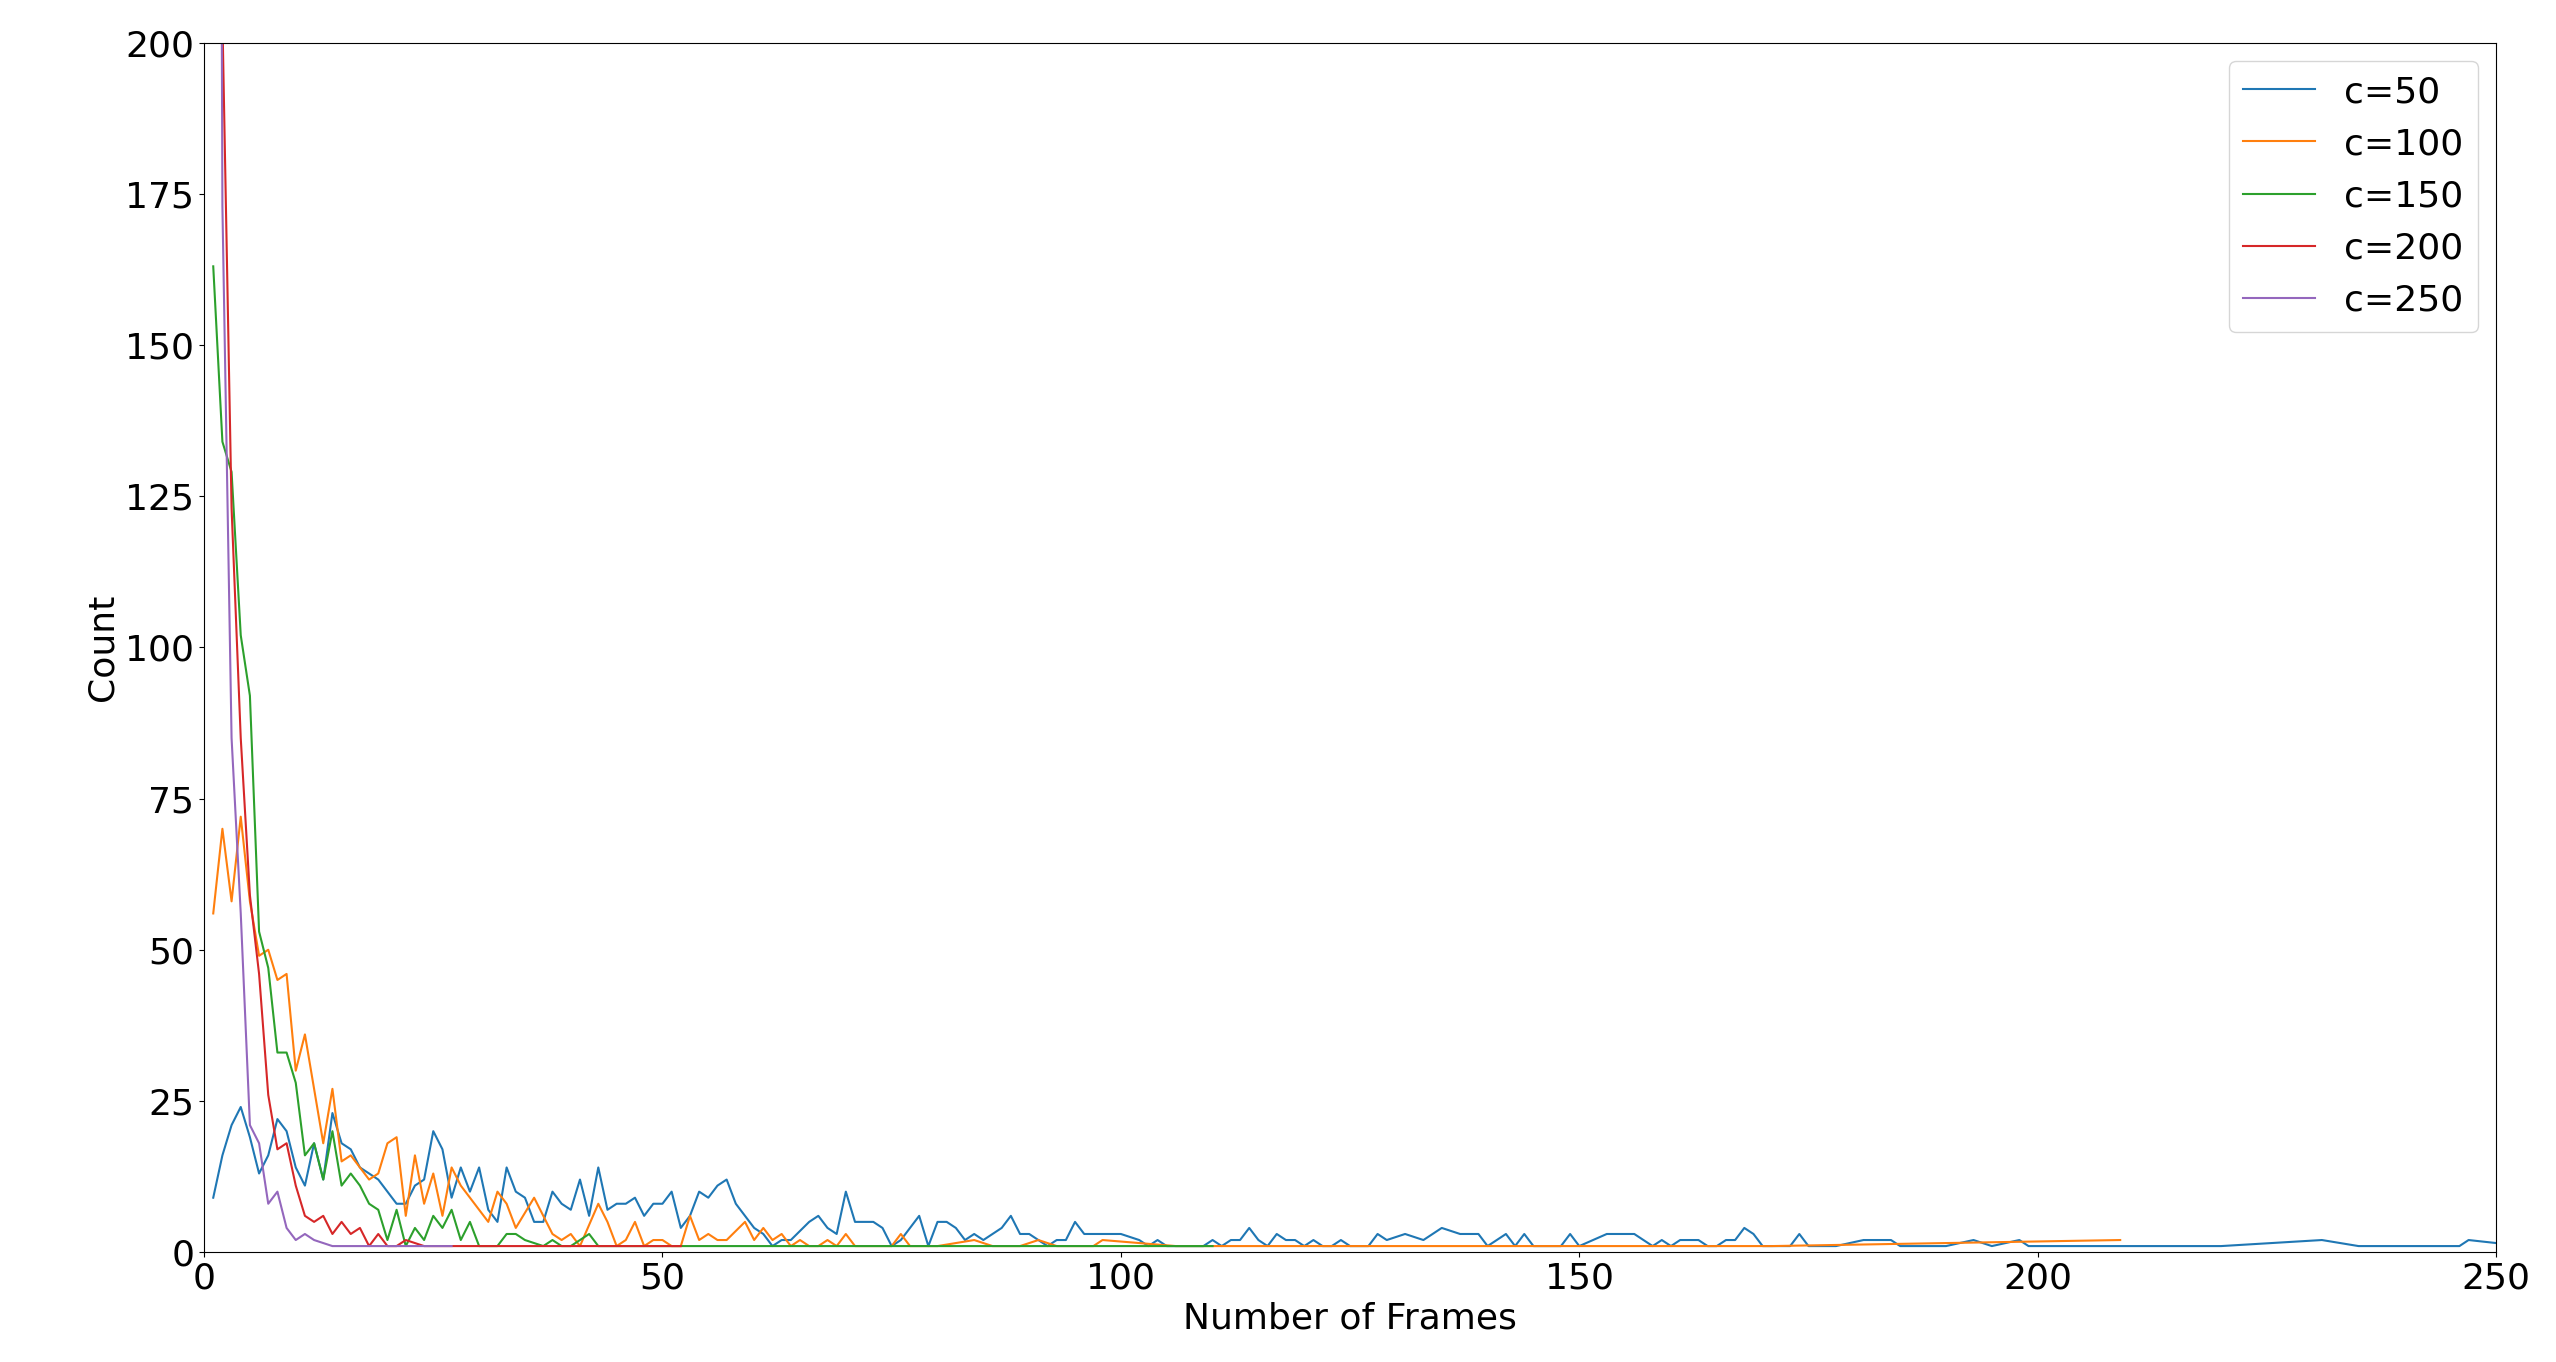
\includegraphics[width=0.8\textwidth]{figures/num_frames_histogram.png}
      \caption{Number of frames selected per video in the MSR-VTT dataset retrieval split when using greedy L1 selection, for different thresholds.}
      \label{fig:optical_flow}
\end{figure}

L1 was chosen over L2 because L2 is very sensitive to large changes in a few pixels; L1 gives a better sense of the overall change in the image.

\section{Prompting Strategies}

The LLM used in testing this pipeline is LLava \cite{llava}.
LLaVA is selected because it is free and open source, and can be run on a single consumer GPU, making it amenable to experimentation.

Beam search, multiple prompts with a temperature.
Two prompts are tried in this work, one of which is is dubbed "concise" (C), while the other is "verbose" (V).
The concise prompt is ""
The verbose prompt is "Please describe the objects in this image. Be as descriptive as possible."
For getting a textual description of a single image, the prompt used is "Please describe the objects in this image. Be as descriptive as possible.".
LLM performance can be sensitive to prompts.

The input to the LLM is a prompt and (potentially) multiple frames, and the output is a text caption.
In all cases, we limit the length of the caption to 512 words, to bound the amount of computation required per frame.

\section{Retrieval}

The last aspect of of the pipeline is, of course, retrieval.
Because LLMs have described the content of the videos at this point in the pipeline, the retrieval task is reduced to that of text retrieval, which is well-studied.
In this work, we explore two retrieval strategies: BM25 and Bi-Encoder, using OpenAI embeddings.
BM25 is a highly performant sparse retriever, relying on term frequencies and other statistics to rank documents.
It is a very fast baseline, retrieving from a thousand documents in milliseconds.

\subsection{Bi-Encoder Retrieval}
This approach is heavily inspired by DPR \cite{dpr}, but uses the same encoder for both documents and queries, and uses L2 distance as a similarity metric instead of the dot product.
In that way, it's similar to the Bi-Encoder strategy used in the BLINK zero-shot entity linker \cite{blink}.
Specifically, the OpenAI model used to generate embedding vectors is \verb|text-embedding-ada-002|, which outputs 1536-dimensional vectors.
The KNN is performed using the FAISS library \cite{faiss}, and all clip descriptions are embedded and stored in an index beforehand, making querying for nearest neighbours very fast.

\begin{figure}
      \centering
      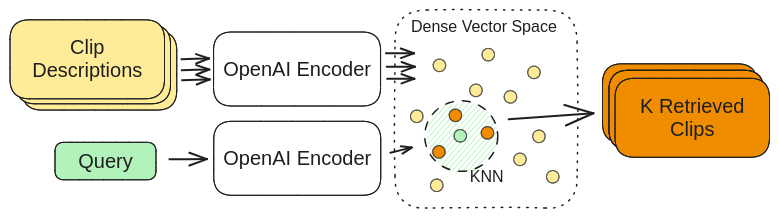
\includegraphics[width=0.8\textwidth]{figures/openai_DPR.png}
      \caption{Bi-Encoder retrieval strategy, using OpenAI embedding API.}
      \label{fig:bienc}
\end{figure}



\section{Results}

\subsection{Video Retrieval}

\begin{table}[htbp]
  \centering
  \begin{tabular}{lccccccc}
    \toprule
    \textbf{Approach} &FS & Prompt & Triple & \multicolumn{3}{c}{\textbf{MSR-VTT} T2V} \\
    \cmidrule(lr){5-7}
                      &&&& \textbf{R@1} & \textbf{R@5} & \textbf{R@10} \\
    \midrule
    CLIP4Clip \cite{clip4clip} &-&-&-& 0.445 & 0.714 &  0.816\\
    \midrule
    X-CLIP \cite{xclip} &-&-&-& 0.493 & 0.758 & 0.848 \\
    \midrule
    InternVideo \cite{internvideo} &-&-&-& 0.552 & - & - \\
    \bottomrule
    VideoDescriptor + BiEnc &5strat&C& & 0.293 & 0.531 & 0.642 \\
    \midrule
    VideoDescriptor + BM25 &5strat&T& & 0.176 & 0.364 & 0.446 \\
  \end{tabular}
  \caption{Performance comparison of the best VideoDescriptor configurations against other models on MSR-VTT T2V retrieval.}
  \label{tab:model_comparison}
\end{table}

The VideoDescriptor pipeline is compared against other models in Table \ref{tab:model_comparison}.
Different configurations of the VideoDescriptor pipeline are compared in Table \ref{tab:video_descriptor_comparison}.
For all MSR-VTT experiments, the videos are considered to be a single clip and thus clip partitioning is not used in the VideoDescriptor pipeline.
Also note that the VideoDescriptor pipeline functions zero-shot, while all other models have been finetuned for text-to-video retrieval using the MSR-VTT training splits.
%Note that due to computational constraints, only the 1000 videos in the MSR-VTT retrieval split were indexed, while in related works the entire test split (a superset of the retrieval split) is indexed.
%As such, direct comparisons between the recall values between this work and related works should not be made.
%Table \ref{tab:model_comparison} is included to provide context for the results of the VideoDescriptor pipeline.
%The retrieval task for the proposed pipeline is much easier, since it is retrieving from a dataset one tenth the size.


\begin{table}[htbp]
  \centering
  \begin{tabular}{lccccccc}
    \toprule
    \textbf{Approach} &Frame Sampling & Prompt & Triplet? & \multicolumn{3}{c}{\textbf{MSR-VTT} T2V} \\
    \cmidrule(lr){5-7}
                      &&&& \textbf{R@1} & \textbf{R@5} & \textbf{R@10} \\
    \midrule
    VideoDescriptor + BiEnc &L1 greedy&V& & 0.215 & 0.439 & 0.544 \\
    \midrule
    VideoDescriptor + BiEnc &3strat&V& & 0.260 & 0.505 & 0.604 \\
    \midrule
    VideoDescriptor + BiEnc &3strat&C& & 0.276 & 0.494 & 0.598 \\
    \midrule
    VideoDescriptor + BiEnc &3strat&T& & 0.265 & 0.480 & 0.590 \\
    \midrule
    VideoDescriptor + BiEnc &3strat&V& \checkmark & 0.269 & 0.505 & 0.604 \\
    \midrule
    VideoDescriptor + BiEnc &3rand&V& & 0.282 & 0.490 & 0.596 \\
    \midrule
    VideoDescriptor + BiEnc &5strat&V& & 0.290 & 0.516 & 0.625 \\
    \midrule
    VideoDescriptor + BiEnc &5strat&C& & \textbf{0.293} & \textbf{0.531} & \textbf{0.642} \\
    \midrule
    VideoDescriptor + BiEnc &5strat&T& & 0.269 & 0.481 & 0.593 \\
    \midrule
    VideoDescriptor + BiEnc &5strat&V& \checkmark & 0.286 & 0.530 & 0.635 \\
    \midrule
    VideoDescriptor + BiEnc &5rand&V& & 0.272 & 0.476 & 0.604 \\
    \bottomrule

    VideoDescriptor + BM25 &L1 greedy&V& & 0.125 & 0.266 & 0.341 \\
    \midrule
    VideoDescriptor + BM25 &3strat&V& & 0.134 & 0.288 & 0.356 \\
    \midrule
    VideoDescriptor + BM25 &3strat&C& & 0.138 & 0.284 & 0.366 \\
    \midrule
    VideoDescriptor + BM25 &3strat&T& & 0.157 & 0.323 & 0.408 \\
    \midrule
    VideoDescriptor + BM25 &3strat&V& \checkmark & 0.122 & 0.277 & 0.347 \\
    \midrule
    VideoDescriptor + BM25 &3rand&V& & 0.142 & 0.280 & 0.340 \\
    \midrule
    VideoDescriptor + BM25 &5strat&V& & 0.167 & 0.326 & 0.411 \\
    \midrule
    VideoDescriptor + BM25 &5strat&C& & 0.150 & 0.331 & 0.417 \\
    \midrule
    VideoDescriptor + BM25 &5strat&T& & \textbf{0.176} & \textbf{0.364} & \textbf{0.446} \\
    \midrule
    VideoDescriptor + BM25 &5strat&V& \checkmark & 0.151 & 0.328 & 0.395 \\
    \midrule
    VideoDescriptor + BM25 &5rand&V& & 0.149 & 0.294 & 0.368 \\
    \midrule
  \end{tabular}
  \caption{Performance of many VideoDescriptor configurations on MSR-VTT T2V retrieval.}
  \label{tab:video_descriptor_comparison}
\end{table}

\subsection{Qualitative Results on Video Summarization}
For visual video summarization, the task is to select a subset of clips from a video relevant to the query, and edit them together into a shorter video.
Sports games are desireable to summarize because they are long, with a few well-defined interesting events (goals, fouls, etc.).
To test this method, a hockey game and a soccer game were partitioned into clips, with each clip being described using \verb|3strat| sampling.
Each clip is described by the LLM using the prompt ``Please describe what is going on in this image".
Then, given a query, the top 30 clips were retrieved using the Bi-Encoder and edited together in order of relevance and rendered into a single video.
The results can be found in the GitHub repository for download: \url{https://github.com/SinclairHudson/video-understanding/tree/main/video_summaries}.

Both the soccer game and hockey game were appproximately 2 hours long, and each video ended up being partitioned into over 700 clips.
The clip partitioning at times struggles with large fast-moving, high contrast objects, which create large inter-frame differences and trigger a clip break.

During retrieval, the VideoDescriptor pipeline struggles to identify semantically meaningful clips, but is able to identify relevant objects easily.
A manual inspection of the descriptions shows that the model is able to describe the frames of the video well, but doesn't get specific about the actions in the scene.
For example, it seems easier for the pipeline to retrieve prompts like ``goaltender", ``referee", or ``coach", and harder to retrieve prompts like ``goal" or ``penalty".
Identifying clips with referees or goaltenders is easy, since they are visually distinct from the rest of the players and easy to identify in an image.

From a runtime perspective, clip partitioning, description, and indexing of a 2-hour sports game takes approximately 4 hours, using an NVIDIA GeForce RTX 3090 GPU for LLM inference.
However, the retrieval step using the FAISS library is very fast, taking less than 170ms to retrieve the top 30 clips from the index.
With more efficient clip partitioning and description, this pipeline could be used to understand videos in practical applications involving video search.


\section{Discussion}

\subsection{Clip Partitioning}

Qualitatively, this approach struggles when large objects move quickly in the video, resulting in large differences between frames.
Additionally, sudden changes in the video, like the flash of a camera, are also often falsely identified as a clip break due to the sudden difference in brightness.
Finally, slow transitions and fade transitions are often not detected because they gradually change from one clip to another.
Transitions found in traditional sports broadcasts can cause such issues.
Those are the 3 most common failure modes of the L1-based clip partitioning algorithm.
In general, false positives will increase the number of clips, and fragment true clips into multiple clips.
Some amount of false positives may be acceptable, depending on the application.
The increased number of clips may slow down the retrieval part of the pipeline, but fragmenting clips may not be problematic.
False negatives are potentially more damaging, creating a segment that is really two clips.
This could potentially unrelated clips into a downstream video summary, for example.

\subsection{Video Retrieval}

At a high level, it would seem that the Bi-Encoder performs better than BM25 for this retrieval task, especially for Recall@1.

For frame selection, it would appear that \verb|5strat| is slightly more performant when compared to equivalent \verb|3strat| experiments, indicating that the extra frames evenly spaced throughout the video are helpful for understanding the video.
The random sampling doesn't perform significantly worse than stratified sampling, contrary to expectation.
This could be due to the fact that the videos in MSR-VTT are relatively short, and so all sampling methods may return very siilar sets of frames for each video.
These videos often only contain one clip, so in this case random sampling isn't prone to catastrophically missing a scene in the video.

For prompt choice, it would seem that this task is relatively insensitive to prompts.
The differences between the concise (C) experiments and equivalent verbose (V) ones are negligible.
However, we do see a significant improvement for the stochastic temperature "prompt" (T), when using the BM25 retriever.
Intuitively this makes sense; a higher temperature will produce a more diverse set of words in the description, which will help tf-idf-based retrievers like BM25 find the right document.

Interestingly, the experiments that use "triple" frames don't perform notably better than the experiments that use single frames in video retrieval.
This seems to suggest that either the additional frames are redundant, or that LLaVA is not good at incorporating information from multiple images in a single generation step.
This is similar to the findings in CLIP4clip, where the authors find that processing frames in batches as 3D tensors doesn't improve performance over frame-by-frame processing \cite{clip4clip}.

The authors of VideoChat note that their similar VideoChat-Text pipeline struggled to understand "intricate temporal reasoning and causal inference".

One interesting feature about the retrieval results of the VideoDescriptor + DPR model is that recall@5 and recall@10 are always the same.
It would seem that if the correct video isn't in the top 5 results, it's not in the top 10 either.
The properties of the OpenAI embedding space aren't well understood, so it's difficult to say why this is the case.



\section{Future work}

Since the VideoDescriptor pipeline has 4 stages and many hyperparameters, there are many avenues for future work.

First and foremost, expanding to other datasets is critical to fully examine the generalization capability of the pipeline.
The current pipeline is currently very slow, requiring many forward passes of a large language model for every frame, and multiple frames for every clip.
It is experimental in nature, and has not been optimized for runtime performance.
With additional engineering effort, the performance of the video processing and text processing elements of the pipeline could both be greatly improved.
Future work could investigate further minimizing the number of frames processed, and prompting techniques to generate very dense captions, with a lot of information content in just a few tokens.

While this work focused on the visual features of video, audio is also often attached to video, and thus could be used to further improve the performance of the pipeline.
Related work such as VideoLLaMA has shown that audio can provide a small boost to performance \cite{videollama}.
Incoporating audio would be particularly important for understanding videos that have an emphasis on dialogue, such as movies.

Future work could also further investigate the influence of prompts and different LLMs on the performance of the pipeline.


\section{Conclusion}

While supervised methods still perform much better than the VideoDescriptor pipeline on text to video retrieval, the VideoDescriptor shows potential for zero-shot retrieval.
Additionally, it can be used for video summarization, and generates compelling videos for queries relating to specific objects in the video.
Hopefully, the performance of the VideoDescriptor pipeline improves as multimodal language models improve.

\bibliographystyle{alpha}
\bibliography{biblio}

\end{document}
